\documentclass[10pt,conference]{IEEEtran}

\usepackage[utf8]{inputenc}
\usepackage{graphicx}
\usepackage{url}
\usepackage{enumitem}
\usepackage{float}

\title{2st Lab with VTK (Visualization Tool Kit)}

\author{
\IEEEauthorblockN{João Varela, 113780}
\IEEEauthorblockN{Carolina Prata, 114246}
\IEEEauthorblockA{Information Visualization, 2025\\
MSc in Computer Engineering, University of Aveiro}
}

\begin{document}

\maketitle

\begin{abstract}
This document provides a brief description of the work developed for the second lab of the Information Visualization course, with the objective of understanding how projections, lighting, and transformations work within VTK.
\end{abstract}

\section{Introduction}
The Visualization Toolkit (VTK) is an open-source software framework extensively used in 3D computer graphics, image processing, and scientific visualization, offering robust tools for handling various data types, supporting visualization methods such as volume rendering, contouring, and streamline analysis, while also enabling the use of multiple actors, renderers, shading options, textures, transformations for object orientation and positioning, and the implementation of observers and callbacks.

\section{Development}

The laboratory assignment provided by the course instructor comprises several exercises covering the following topics:

\begin{itemize}
    \item Multiple actors;
    \item Multiple renderers;
    \item Shading options;
    \item Textures;
    \item Transformations;
    \item Observers and callbacks;
\end{itemize}


\subsection{Multiple actors}
For the first exercise, it was required to add multiple actors to one render in \texttt{cone.py}. In this case, we were asked to create two identical cones with different colors. We used two approaches to manipulate the properties of each cone: in the first case, we set each property individually, while in the second case, we created a \texttt{vtkProperty} to store and modify the properties and then assigned it to the actor. Additionally, we were asked to set the opacity of both cones to 0.5.
We changed the background to white \texttt{SetBackground(1.0, 1.0, 1)} to better visualize the different opacities.


The following code demonstrates how we set the properties of the first cone individually:

{\small
\begin{verbatim}
coneActor.GetProperty().SetColor(0.2, 0.63, 0.79)
coneActor.GetProperty().SetDiffuse(0.7)
coneActor.GetProperty().SetSpecular(0.4)
coneActor.GetProperty().SetSpecularPower(20)
coneActor.GetProperty().SetOpacity(0.5)
\end{verbatim}
}


For the second cone, we used a \texttt{vtkProperty} to store and modify the properties, which were then applied to the actor. We also set its position to \texttt{(0, 2, 0)}:

\begin{verbatim}
property = vtkProperty()
property.SetColor(1.0, 0.3882, 0.2784)
property.SetDiffuse(0.7)
property.SetSpecular(0.4)
property.SetSpecularPower(20)
property.SetOpacity(0.5)

coneActor2 = vtkActor()
coneActor2.SetMapper(coneMapper)
coneActor2.SetPosition(0, 2, 0)
coneActor2.SetProperty(property)
\end{verbatim}

Both cones were given an opacity of 0.5, resulting in a semi-transparent effect. The second cone was also translated by 2 units along the Y-axis, as seen in the \texttt{SetPosition} method.

\begin{figure}[H]
\centering

\begin{minipage}{0.45\columnwidth}
    \centering
    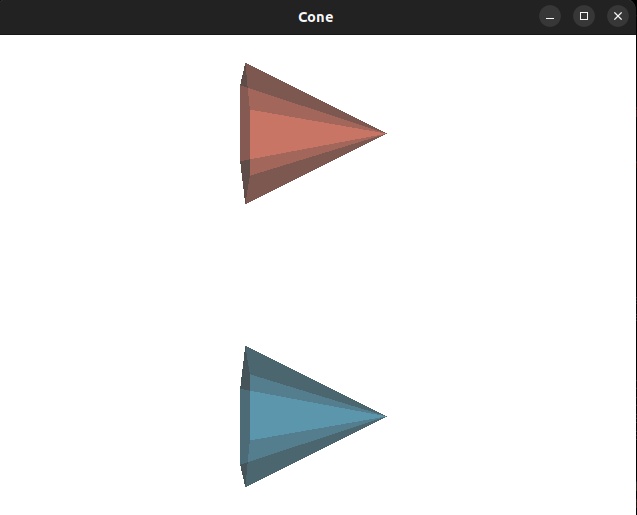
\includegraphics[width=\linewidth]{lesson2/fig1_50opc.png}
    
\end{minipage}
\hfill
\begin{minipage}{0.45\columnwidth}
    \centering
    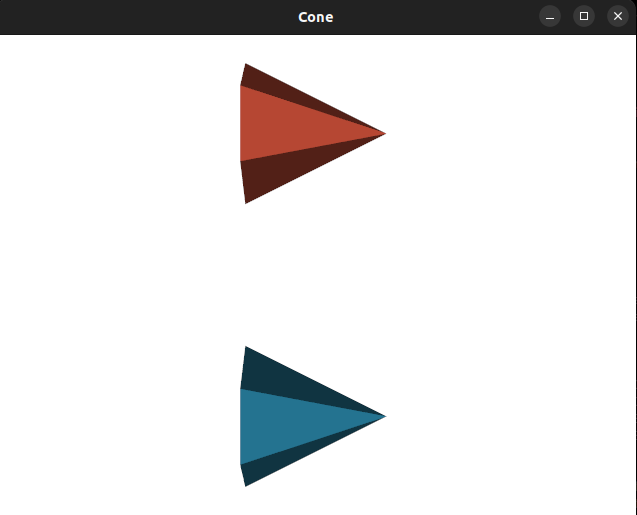
\includegraphics[width=\linewidth]{lesson2/fig1_normal.png}
\end{minipage}

\caption{Comparison of the cone's appearance with reduced opacity (0.5) and full opacity (1).}

\end{figure}

We concluded that by reducing the opacity, the other faces of the cones became visible, giving the appearance of acrylic. Apart from this, the application of properties produced the same result regardless of the method used to modify them for each cone.

\subsection{Multiple renderers}
This exercise involved displaying two renderers within a single window, done in \texttt{renderers.py}. To achieve this, we used the cone example from the previous lab and divided the window (set to 600 x 300 pixels) into two sections using the SetViewport method. The second renderer's camera was rotated 90 degrees in azimuth. Additionally, we modified the background colors for each renderer to better distinguish them.

\begin{figure}[H]
\centering
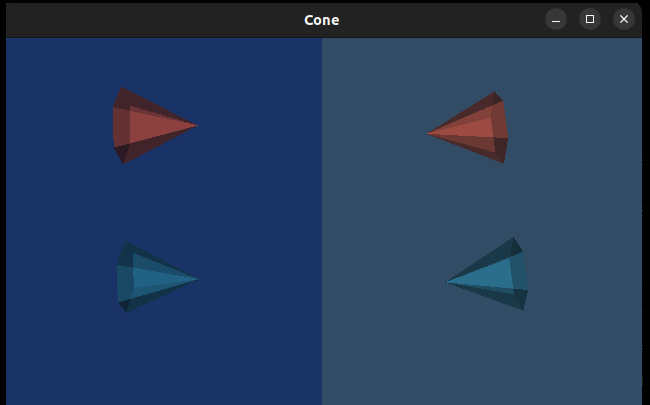
\includegraphics[width=0.40\textwidth]{lesson2/fig2.png}
\caption{Result of the execution of the double renderer.}
\end{figure}



\subsection{Shading options}

For this exercise, done in \texttt{shadings.py}, the cones were replaced by spheres in order to explore and apply different shading techniques available in VTK. To make the differences between shading models more noticeable, the sphere resolution was reduced by setting both the \texttt{PhiResolution} and \texttt{ThetaResolution} to 10. Instead of using two renderers and two spheres as initially required, we implemented four renderers, each displaying a single sphere. 

Each renderer was configured with a different shading model: one sphere used the default shading, while the remaining spheres were rendered using \texttt{SetInterpolationToFlat}, \texttt{SetInterpolationToGouraud}, and \texttt{SetInterpolationToPhong}, respectively. 

This setup allowed for a direct visual comparison of the effects produced by each shading method.

\begin{figure}[H]
\centering

\includegraphics[width=0.40\textwidth]{lesson2/fig3.png}
\caption{ Result of the execution of the shading exercise.}
\end{figure}

We observed that VTK applies Gouraud shading by default. The results showed that Gouraud and Phong shading often produce similar visual outcomes; however, Phong shading generally provides smoother lighting transitions and more realistic specular highlights. In contrast, flat shading is the most visually distinct, as it applies uniform lighting to each polygon, resulting in a clearly faceted appearance.

\subsection{Textures}
In this exercise, a plane was created using \texttt{vtkPlaneSource} and textured with an image in \texttt{textures.py}. The plane was defined as a 10×10 square by specifying an origin at $(0,0,0)$ and two edge points at $(10,0,0)$ and $(0,10,0)$. The Lena image was loaded using \texttt{vtkJPEGReader} and applied to the plane through a \texttt{vtkTexture} object. The texture was then assigned to the plane’s actor using \texttt{SetTexture()}, mapping the image onto the surface and allowing it to be rendered correctly within the scene.

The result was a plane with the image as the texture as follows:

\begin{figure}[H]
\centering
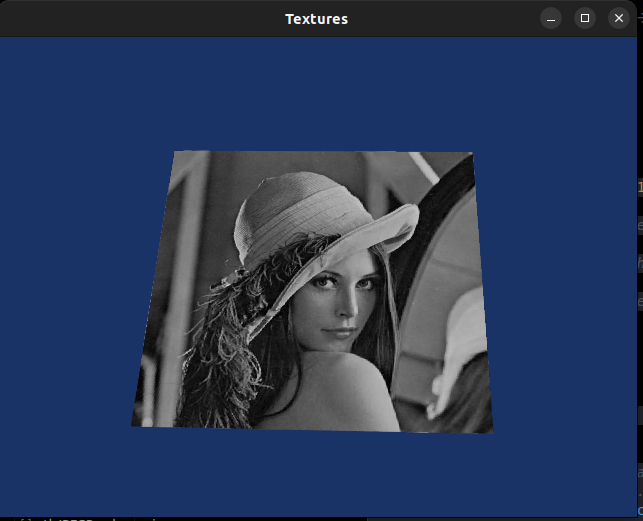
\includegraphics[width=0.40\textwidth]{lesson2/fig4.png}
\caption{Result of the execution of the transformation exercise.}
\end{figure}

When the dimensions of the plane are modified using the \texttt{SetOrigin}, \texttt{SetPoint1}, and \texttt{SetPoint2} methods, the applied texture automatically scales to cover the entire surface of the plane. As a result, the texture stretches or compresses to fit the new geometry, regardless of the plane’s size or aspect ratio

\begin{figure}[H]
\centering
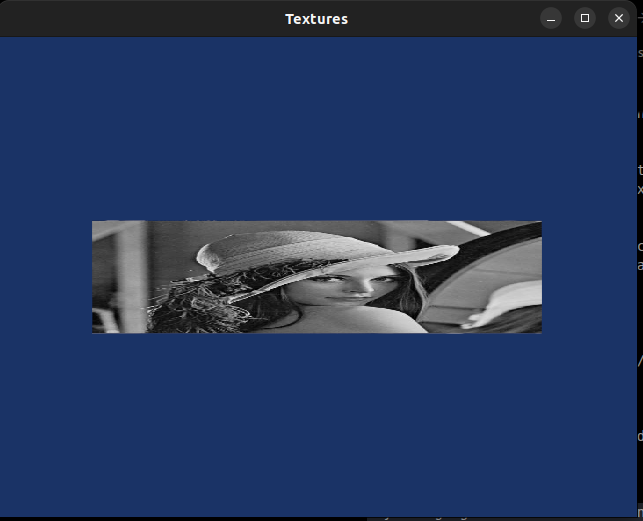
\includegraphics[width=0.40\textwidth]{lesson2/fig4.1.png}
\caption{Result of the execution of the transformation exercise.}
\end{figure}

\vspace{0.1cm}

\subsection{Transformations}
This exercise demonstrates the construction of a textured cube in VTK using individual planar faces in \texttt{transformations.py}. Each face of the cube is generated through a dedicated function, \texttt{render\_cube\_face}, which creates a plane and applies the necessary geometric transformations to position it correctly in 3D space. The transformations are performed using \texttt{vtkTransform}, combining rotations and translations to orient and place each face. Rotations are defined using an angle--axis representation, where the rotation angle is specified in degrees and the axis is defined by a three--component vector.

The transformed geometry is processed using \texttt{vtkTransformPolyDataFilter}, which applies the transformation to the polygonal data. For texture mapping, \texttt{vtkJPEGReader} is used to load an image for each face, and \texttt{vtkTexture} applies the corresponding texture to the plane. By creating six planes with distinct transformations and textures, a complete cube is assembled, with each face displaying a different image.

\begin{figure}[H]
\centering

\includegraphics[width=0.40\textwidth]{lesson2/fig5.png}
\caption{ Result of the execution transformations.py file}
\end{figure}

\subsection{Observers and callbacks}

In the final part of the lab, we explored VTK’s mechanism for defining callback functions and associating them with objects through observers. To achieve this, a new file named \texttt{callbacks.py} was created based on the cone example from the first lab. A custom callback class, \texttt{vtkMyCallback}, was implemented to react whenever a specified event occurs during the rendering process.

When an event is triggered, the callback prints diagnostic information to the terminal, including the class name of the object that generated the event, the event type, and the current camera position in 3D space. By registering the callback with \texttt{vtkCommand.AnyEvent}, it was possible to capture and log multiple events occurring throughout the rendering cycle, such as \texttt{StartEvent}, \texttt{EndEvent}, \texttt{ModifiedEvent}, and \texttt{ResetCameraClippingRangeEvent}.

The observed output shows that \texttt{StartEvent} is triggered at the beginning of each rendering cycle, while \texttt{EndEvent} occurs once rendering is complete. By changing the observer to listen only to specific events (e.g., \texttt{vtkCommand.StartEvent}, \texttt{vtkCommand.EndEvent}, or \texttt{vtkCommand.ResetCameraEvent}), the callback mechanism can be tailored to respond selectively, enabling fine-grained control over event handling and effective debugging within the VTK rendering pipeline.


\end{document}
